\documentclass[a4paper, 12 pt]{article}

\usepackage{graphicx, float}
\usepackage{fourier}
\usepackage[french]{babel}
\usepackage[T1]{fontenc}
\usepackage[utf8]{inputenc}

\title{\LARGE \textbf{LES VUES MULTIPLES D'UN SOLIDE}}
\author{MATH\'EMATHIQUES 5P}
\date{\today}



\begin{document}

    \Large
    

    \begin{titlepage}
        
        \maketitle
    \end{titlepage}
    
    \setcounter{page}{2}

    %\tableofcontents

    %\newpage

    \section{Vue de gauche}

    \begin{figure}[H]
        \centering
        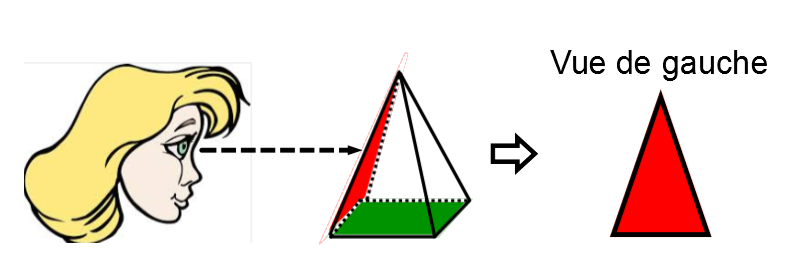
\includegraphics[width = 1\linewidth]{vueGauche.PNG}
        \caption[]{Visualiser le solide depuis la gauche}
    \end{figure}

    
    Exercices :

   

    
    
\end{document}
